\epigraph{\emph{
  ``All models are wrong, but some are useful.''
}}{ George E. P. Box }

\section{Summary}
\label{sec:summary}
Summing up all the pieces, this thesis provided a starting point of building a robust  news article summarization system. The groundwork on different clustering strategies were examined and several techniques of transformation from documents, to words, to coincidence matrices to statistical topical proportions were investigated. We heard a lot about feature selection and semantics, as well as different strategies on how to deal with word sense disambiguation. It was concluded that most of the strategies perform well but that the simplest of all models, namely by using the word tokens of a document, was superior to other approaches. Furthermore the data pipeline ``News-Clusty'' was evaluated and depicted. Several steps are necessary to get a vector of features from a real world document. Dealing with the noise and with the time drift effects by statistical techniques such as \lsa{} or \lda{} showed promising results. At last, we have shown how the clustering algorithm works on the BBC dataset and experimented, without giving any evidence, how the system works on real world data.

\section{Further Reading / Related Work}
\label{sec:further_reading}
In this section it is important to distinguish between the data pipeline and the quality of the algorithmic procedures. A generally well composed article about the different current approaches to clustering large and small documents is \cite{NextFrontierClustering2013}.\\

Several models of topic models were examined. There is more room to study the effects of \lda{} and certainly trying \hdp{}. For multi document summarization \lda{} can be used as a main approach, see \cite{MultiDocSumLDA2008}. The concepts of \hdpfull{} can be found in \cite{NonParametricBayes2007, HDP2006}. Further we could use Non-negative matrix factorization (NMF) as a matrix decomposition technique. See \cite{NMF1999} for a proper introduction.\\

While completely using unsupervised learning we could use artificial neural networks as well. A promising approach is the shallow neural network word2vec, that learns a feature representation using skip-gram models. See \cite{Word2Vec2014} for a good introduction.\\

Enhancing feature selection methods and more semantic relations promising work was done by \cite{NounPhraseSemanticClustering@2009@Zheng} using noun phrases for semantic clustering and 
\cite{WordNetAndFuzzyAssociation@2010@Chen} with \wordnet{} and soft assignment clustering. Further we can investigate external knowledge sources like \wiki{} to boost feature selection. Some good approaches were found in \cite{WikipediaClusteringSim2009} and \cite{WikipediaClustering2010}.\\

Time series clustering could not be tackled in this thesis. Beginning with basic introductions see \cite{ClusteringTimesSeriesSurves2005, RecentTechniquesClusteringSurvey2012, IncrementalClustering2012}. A good starting point for understanding topic models over time is \cite{BlogTopicLDA2013} analyzing blog posts.\\

The data pipeline is analogous to the Columbia Newsblaster System by \cite{NewsBlaster2002}. The whole literature evolving on the system is a vantage point for further reading. Also everything around the Google News aggregation system exemplified by \cite{GoogleNews2007}.\\

At last we have to mention the scalability issues. Working with algorithms across several server nodes needs different techniques. Algorithms need to be parallelized by techniques like map reduce, see \cite{MapReduce2008}. See parallel clustering approaches by \cite{ParallelClustering2009}.

\section{Future Work}
\label{sec:future_work}
Future work needs to be done on several things in the data pipeline.

\begin{description}
  \item[First] scaling and enhancement for data sets. This includes adding more newspaper data. In reality the classification system for news categories needs to be normalized across all newspapers. Finding ways of detecting the label of a document when downloading an article.
  \item[Second] adding a multi-document summarization system that works with the clustering.
  \item[Third] a routing system that detects the kind of event by biographical, single and multi events.
  \item[Fourth] scaling the clustering algorithms to several days by strategies mentioned in the experimental multiple days section.
  \item[Fifth] adding more feature selection strategies with \wordnet{}, \wiki{} and word2vec.
  \item[Sixth] using more advanced algorithms, especially topic modeling and semi supervised kernel methods.
  \item[Seventh] including external knowledge sources that work during the clustering methods as well.
  \item[Eighth] using state of the art distributed file systems to ease the task of feature selection and clustering
\end{description}

None of the above tasks is trivial. Each would greatly enhance the systems performance and usability. In theory the accuracy can be enhanced by incorporating more reliable and complex models to the clustering task. In total the system could be further prepared to run on international data sets from official conferences. A compact evaluation of the status quo against other systems was currently not possible. The status of the system is still in alpha stadium and thus, not production ready.

\subsection*{Multiple days clustering}
  The proposed model, seen in figure \ref{time_clustering}, is by clustering consecutive days without any overlap. After this, all cluster centers are consecutively merged and reassigned. The merging is based on similarity thresholds. If the similarity is high enough or we find hard evidence, like a named entity, cluster centers can be merged. Otherwise the clusters are kept separate. Going further we can set hard thresholds, how old a cluster should be, before it is not being considered anymore. Deciding when a merge, a reassignment or a new cluster emerges is the goal.

    \begin{figure}[h!]
      \centering
        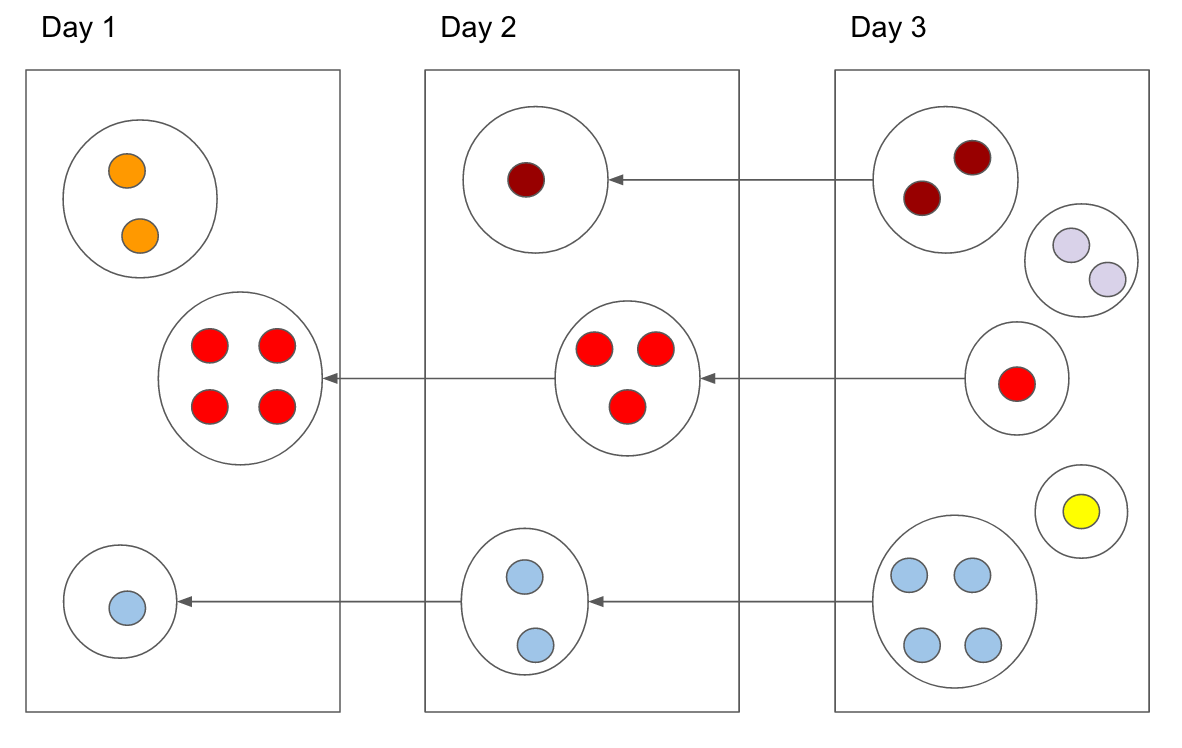
\includegraphics[width=0.7\textwidth]{time_clustering.png}
        \caption{"Multiple days clustering consecutive"}
        \label{time_clustering}
    \end{figure} 

  Several important enhancements to single day clustering must be made.

  \begin{description}
    \item[First] we need timestamps for each document
    \item[Second] we need to track documents over the course of several days. As the document size grows, algorithms need to be rethought for online or batch variations. In \cite{BlogTopicLDA2013} is a comprehensive analysis of blogs over time using \lda{}.
    \item[Third] solutions to over fitting must be found. That is, assigning too many documents to an existing cluster center.
    \item[Fourth] biasing must be avoided by inflating clusters that are of the same topics.
    \item[Fifth] measures have to be rethought. The silhouette coefficient will grow small with more documents in vector space. Different results are not comparable.
  \end{description}

  The content of this section is open for future work. Later we will discuss some articles dealing with the problem.

\section{Final Words}
We conclude this thesis with a quote of George E. P. Box, \emph{``All models are wrong, but some are useful.''}. I find this especially true for a domain, where text is seen as a system of linear combinations. In this sense, thank you very much for reading.

